\documentclass[10pt]{article}
\usepackage[a4paper,margin=0.6in]{geometry}
\usepackage[T1]{fontenc}
\usepackage{times}
\usepackage{microtype}
\usepackage{booktabs,tabularx,array}
\usepackage{enumitem}
\usepackage{titlesec}
\usepackage{float}
\usepackage{caption}
\usepackage{xcolor}
\usepackage{tikz}
\usetikzlibrary{positioning,arrows.meta}
\usepackage[hidelinks]{hyperref}
\titleformat{\section}{\normalsize\bfseries}{\thesection}{0.5em}{}
\titlespacing*{\section}{0pt}{5pt}{2pt}
\titleformat{\subsection}{\small\bfseries}{\thesubsection}{0.5em}{}
\titlespacing*{\subsection}{0pt}{3pt}{1pt}
\setlist{nosep,leftmargin=1.2em}
\setlength{\parskip}{2pt}
\setlength{\parindent}{0pt}
\renewcommand{\arraystretch}{1.05}
\newcolumntype{Y}{>{\raggedright\arraybackslash}X}
\captionsetup{font=small,skip=2pt}
\begin{document}

\begin{center}
{\LARGE\bfseries Knowing When Not to Answer}\\[3pt]
{\large\bfseries Abstention Drift in Multi-Turn Retrieval-Augmented Conversations}\\[4pt]
{\small CS683 -- Natural Language Processing \,|\, Course Project Report \,|\, October 2026}\\[2pt]
{\small Indian Institute of Information Technology Guwahati \,\textbullet\, Code: \url{https://github.com/SK-099/abstention-drift}}
\end{center}
\vspace{-4pt}
\begin{table}[H]
\centering\small
\begin{tabular}{@{}lll@{}}
\toprule
Name & Roll No. & E-mail \\
\midrule
Arpan Mondal & 2521505 & arpan.mondal25m@iiitg.ac.in \\
Abhilash Basumatary & 2521501 & abhilash.basumatary25m@iiitg.ac.in \\
Poulami Mukherjee & 2521524 & poulami.mukherjee25m@iiitg.ac.in \\
Subhashis Kar & 2521538 & subhashis.kar25m@iiitg.ac.in \\
Kadapala Goharsh Reddy & 2521516 & kadapala.reddy25m@iiitg.ac.in \\
\bottomrule
\end{tabular}
\caption{Project group.}
\end{table}
\vspace{-10pt}

\section{Introduction}
Chat assistants that answer from a user's own documents use retrieval-augmented generation (RAG) \cite{rag}: they retrieve passages and let a language model answer from them. Their most harmful failure is answering confidently when the documents do \emph{not} contain the answer. The goal of this project was to build and deploy a complete, self-hosted notebook assistant that (i) answers only from the user's sources, with citations, (ii) says ``I don't know'' when the sources do not support an answer, also late in a long conversation, and (iii) runs on modest hardware: a laptop with a 4\,GB GPU and a free-tier cloud virtual machine. The project was carried out in two stages: a research stage that measured abstention on the MTRAG-UN benchmark and chose the refusal method, and an engineering stage that turned the result into the deployed application described in this report.

\section{Related Work}
SQuAD~2.0 \cite{squad2} made unanswerable questions a standard test, and RGB \cite{rgb} showed that RAG models often answer from irrelevant passages. Surveys of abstention \cite{wen2025} and multi-model approaches \cite{feng} study when a model should decline; selective prediction \cite{selective,kamath} chooses refusal thresholds under a risk budget, the approach we use for every model. Self-RAG \cite{selfrag} checks its own answers, similar to our self-check step. MTRAG \cite{mtrag} and MTRAG-UN \cite{mtragun} provide multi-turn RAG conversations with unanswerable questions; at SemEval-2026 a strong system still detected only 21.8\% of them on the development set \cite{ails}. Existing source-grounded notebook assistants are mostly closed, cloud-only services; our application provides this workflow with open models that run locally.

\section{Problem Definition}
Given a notebook of sources (PDFs, web pages, YouTube transcripts, pasted text) and a conversation, the assistant must, at every turn, either give an answer whose statements are supported by cited passages, or refuse. The requirements for the deployed system were:
\begin{itemize}
\item \textbf{Grounded, cited answers} and a measured, low rate of both wrong answers to unanswerable questions (\emph{abstain recall}) and wrong refusals of answerable ones (\emph{false-abstention rate}, FA).
\item \textbf{Choice of model}: ten free open-weight models (1--4B parameters, via Ollama), each with its own refusal thresholds, since models differ strongly in how often they refuse on their own.
\item \textbf{Notebook features}: source guides, notebook-wide summaries, Studio outputs (briefing, study guide, FAQ, timeline, mind map, flashcards, quiz, two-voice audio overview), notes and sharing.
\item \textbf{Deployability}: one-command start with Docker Compose on a laptop and on an AWS EC2 instance, with automated tests on every change.
\end{itemize}

\section{Experiments and Results}
\subsection{System built}
The assistant is a LangGraph agent behind a FastAPI service (Figure~\ref{fig:arch}). For each question it rewrites the question using the chat history, runs hybrid search (BM25 \cite{bm25} and BGE embeddings \cite{bge} fused with reciprocal rank fusion \cite{rrf}, then a cross-encoder re-ranker \cite{monobert}) over the notebook's passages in Qdrant, and scores answerability with a fine-tuned checker (gate). It abstains if the gate score $p\ge\tau$, if the model itself refuses, or if $p\ge$ min\_p and a self-check finds the answer unsupported; before refusing it searches once more with a rewritten query. A Celery worker indexes sources and generates Studio outputs; Kokoro text-to-speech voices the audio overview.

\begin{figure}[H]
\centering
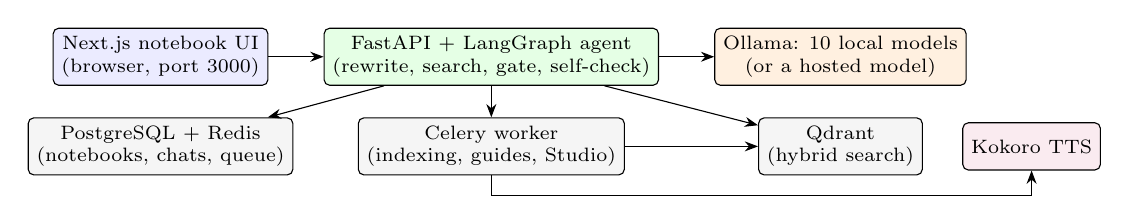
\begin{tikzpicture}[font=\scriptsize, >=Stealth,
 box/.style={draw, rounded corners=2pt, align=center, inner sep=3pt, minimum height=6mm, fill=#1}, box/.default=gray!8]
\node[box=blue!8] (web) {Next.js notebook UI\\(browser, port 3000)};
\node[box=green!10, right=7mm of web] (api) {FastAPI + LangGraph agent\\(rewrite, search, gate, self-check)};
\node[box=orange!12, right=7mm of api] (llm) {Ollama: 10 local models\\(or a hosted model)};
\node[box, below=4mm of web] (db) {PostgreSQL + Redis\\(notebooks, chats, queue)};
\node[box, below=4mm of api] (wk) {Celery worker\\(indexing, guides, Studio)};
\node[box, below=4mm of llm] (q) {Qdrant\\(hybrid search)};
\node[box=purple!8, right=5mm of q] (tts) {Kokoro TTS};
\draw[->] (web)--(api); \draw[->] (api)--(llm); \draw[->] (api)--(wk); \draw[->] (api)--(db); \draw[->] (api)--(q); \draw[->] (wk)--(q); \draw[->] (wk.south) -- ++(0,-2.5mm) -| (tts.south);
\end{tikzpicture}
\caption{Architecture of the deployed application (all parts run as Docker containers; Ollama runs on the host).}
\label{fig:arch}
\end{figure}
\vspace{-6pt}

\subsection{Choosing the refusal method}
On the MTRAG-UN test set (429 turns, 97 unanswerable) we compared a fixed pipeline with answerability gates and with the agent (Table~\ref{tab:method}). Detection of unanswerable questions did not get worse in later turns (all slopes near zero, confidence intervals contain zero), so no turn-specific fix was needed. The main weakness was \emph{over-refusal}; the agent's ``search again before refusing'' step lowered it to 13.6\%, and adding the calibrated self-check gave the best F1, so this configuration was deployed.

\begin{table}[H]
\centering\small
\begin{tabular}{@{}lccccl@{}}
\toprule
Configuration (Qwen2.5-3B) & F1 & Abstain recall & Precision & FA $\downarrow$ & Recall change per turn [95\% CI] \\
\midrule
Hybrid retrieval, prompt-only refusal & .443 & .464 & .425 & .184 & $-$.003 [$-$.046, +.043] \\
+ fine-tuned answerability gate & .449 & .495 & .410 & .208 & +.008 [$-$.034, +.051] \\
Agent: retry before refusing & .465 & .443 & \textbf{.489} & \textbf{.136} & +.010 [$-$.033, +.054] \\
\textbf{Agent: retry + self-check (deployed)} & \textbf{.511} & \textbf{.577} & .459 & .199 & +.020 [$-$.026, +.068] \\
\bottomrule
\end{tabular}
\caption{Abstention on MTRAG-UN (429 turns).}
\label{tab:method}
\end{table}
\vspace{-6pt}

\subsection{Per-model refusal thresholds}
For each of the ten models we chose $(\tau,\text{min\_p})$ on 224 MTRAG development turns to maximise F1 while keeping FA at most 10 points above the model's own refusal rate. The best models reached F1 .67 (Gemma-3-4B, Qwen3-1.7B) against .62 for the research model Qwen2.5-3B; the best thresholds ranged from $\tau=.45$ to $.64$, which confirms that one setting cannot serve all models. The model menu marks calibrated models with a shield.

\subsection{End-to-end testing}
A test script drives the running application through its API exactly as the interface does. It was run on the laptop with three research papers and all ten models (Table~\ref{tab:e2e}); continuous integration on GitHub additionally runs lint, 88 unit tests, the web build and an abstention quality gate on every push.

\begin{table}[H]
\centering\small
\begin{tabularx}{\textwidth}{@{}lYl@{}}
\toprule
Feature tested (all 10 models) & Result & Status \\
\midrule
Chat: answerable questions & 48/60 answered with citations to the right sections (experiments questions cite Experiments/Results) & pass \\
Chat: unanswerable questions & 26/30 refused; only DeepSeek-R1-1.5B and SmolLM2-1.7B (own refusal rate .09/.02) answered & pass \\
Sources & PDF, web page, pasted text, YouTube (timestamped citations), web search; source guides & pass \\
Studio & briefing, study guide, FAQ, timeline, mind map, flashcards, quiz; audio overviews of 60--230\,s & pass \\
Sharing and notes & viewer/editor roles, link access and revoking tested with separate users; notes stay private & pass \\
Overall & 184 checks in the main run, 0 failures; 22 warnings were model behaviour, not faults & pass \\
\bottomrule
\end{tabularx}
\caption{End-to-end test results.}
\label{tab:e2e}
\end{table}
\vspace{-6pt}

\subsection{Deployment}
\begin{table}[H]
\centering\small
\begin{tabularx}{\textwidth}{@{}lYY@{}}
\toprule
 & Laptop & AWS EC2 (free-plan credits) \\
\midrule
Hardware & 16\,GB RAM, NVIDIA GTX 1650 (4\,GB) & \texttt{m7i-flex.large}: 2 vCPU, 8\,GB RAM, 40\,GB disk, no GPU \\
Models & all 10 local models & 7 small models chosen for CPU speed and disk space \\
Typical answer time & 10--70\,s & tens of seconds (CPU only) \\
Access & \url{http://localhost:3000} & public IP, ports limited to the team's addresses \\
Cost & -- & about USD 0.10 per hour; stopped when not in use \\
\bottomrule
\end{tabularx}
\caption{Deployment environments.}
\end{table}
\vspace{-6pt}
\textbf{Problems found and fixed during deployment.} Ollama's default 4{,}096-token window silently cut the sources out of long Studio prompts, so small models wrote about unrelated topics (fixed with a larger window for long jobs and an off-topic check); reference lists of papers were retrieved as evidence (filtered); several containers each using all CPU threads slowed answers about tenfold (thread limits); and the web interface needs the server's public address at build time, which is documented in the deployment guide.

\section{Conclusion}
We built and deployed a self-hosted notebook assistant that answers from the user's sources with citations and refuses when they do not support an answer. Measurements on MTRAG-UN guided the design: abstention does not drift over a conversation, the real problem is over-refusal, and an agent that searches again and checks its answer gives the best balance (F1 .511). Per-model thresholds make ten open models usable, and the end-to-end test passed for all of them on a laptop, with the system also running on an AWS free-plan instance. Remaining limitations are slow CPU-only answers in the cloud, no sign-in for public use, and a gate that is less reliable on scientific papers than on the domains it was trained on; calibrating the gate on users' own documents and adding authentication are the next steps.

\clearpage
\begin{thebibliography}{99}\setlength{\itemsep}{1pt}\small
\bibitem{mtrag} Y.~Katsis, S.~Rosenthal, et al. MTRAG: A Multi-Turn Conversational Benchmark for Evaluating Retrieval-Augmented Generation Systems. \emph{TACL} 13:784--808, 2025.
\bibitem{mtragun} S.~Rosenthal, Y.~Katsis, et al. MTRAG-UN: A Benchmark for Open Challenges in Multi-Turn RAG Conversations. \emph{Findings of ACL 2026}, pp.~10363--10369, 2026.
\bibitem{ails} D.~Athanasiou, M.~Lymperaiou, G.~Filandrianos, A.~Voulodimos, G.~Stamou. AILS-NTUA at SemEval-2026 Task 8: Evaluating Multi-Turn RAG Conversations. \emph{Proc.\ SemEval-2026}, pp.~1340--1365, 2026.
\bibitem{rag} P.~Lewis et al. Retrieval-Augmented Generation for Knowledge-Intensive NLP Tasks. \emph{NeurIPS}, 2020.
\bibitem{squad2} P.~Rajpurkar, R.~Jia, P.~Liang. Know What You Don't Know: Unanswerable Questions for SQuAD. \emph{ACL}, 2018.
\bibitem{rgb} J.~Chen, H.~Lin, X.~Han, L.~Sun. Benchmarking Large Language Models in Retrieval-Augmented Generation. \emph{AAAI}, 2024.
\bibitem{wen2025} B.~Wen et al. Know Your Limits: A Survey of Abstention in Large Language Models. \emph{TACL} 13, 2025.
\bibitem{feng} S.~Feng et al. Don't Hallucinate, Abstain: Identifying LLM Knowledge Gaps via Multi-LLM Collaboration. \emph{ACL}, 2024.
\bibitem{selective} Y.~Geifman, R.~El-Yaniv. Selective Classification for Deep Neural Networks. \emph{NeurIPS}, 2017.
\bibitem{kamath} A.~Kamath, R.~Jia, P.~Liang. Selective Question Answering under Domain Shift. \emph{ACL}, 2020.
\bibitem{selfrag} A.~Asai et al. Self-RAG: Learning to Retrieve, Generate, and Critique through Self-Reflection. \emph{ICLR}, 2024.
\bibitem{bm25} S.~Robertson, H.~Zaragoza. The Probabilistic Relevance Framework: BM25 and Beyond. \emph{Foundations and Trends in IR}, 2009.
\bibitem{bge} S.~Xiao et al. C-Pack: Packed Resources for General Chinese Embeddings. \emph{SIGIR}, 2024.
\bibitem{rrf} G.~Cormack, C.~Clarke, S.~B\"uttcher. Reciprocal Rank Fusion Outperforms Condorcet and Individual Rank Learning Methods. \emph{SIGIR}, 2009.
\bibitem{monobert} J.~Lin, R.~Nogueira, A.~Yates. \emph{Pretrained Transformers for Text Ranking: BERT and Beyond}. Synthesis Lectures on Human Language Technologies, Morgan \& Claypool, 2021.
\end{thebibliography}
\end{document}
